\documentclass{article}
\usepackage{amsmath, amssymb, mathtools, verbatim, tikz, graphicx,nicefrac}
\usepackage[margin=0.5in]{geometry}
\graphicspath{{images/}}
\setlength{\parindent}{0pt}
\renewcommand{\t}[1]{\text{#1}}
\newcommand{\N}{\mathbb{N}}
\newcommand{\sumx}[2]{\sum\limits_{#1}^{#2}}
\newcommand{\ord}{\text{ord}}
\newcommand{\frp}{\text{FRP}}
\newcommand{\R}{\Rightarrow\,}
\newcommand{\B}[1]{\textbf{#1}}
\newcommand{\I}{\bigcap}
\newcommand{\U}{\bigcup}
\newcommand{\V}{\vert}
\newcommand{\F}[1]{\lfloor#1\rfloor}
\renewcommand{\t}[1]{\text{#1}}
\newcommand{\lra}[1]{\langle#1\rangle}
\newcommand{\len}[1]{\vert#1\vert}
\newcommand{\num}{\text{num}}
\newcommand{\nfrc}[2]{\nicefrac{#1}{#2}}
\begin{document}
\begin{center}
  21--499 Chess Game
\end{center}
\paragraph{Describing The Game}\mbox{}\\
Suppose we have a chessboard, and there's a knight somewhere on this
chessboard. The location of the knight is indicated by a blue square.
As an example consider the drawing below: \\
\begin{center}
  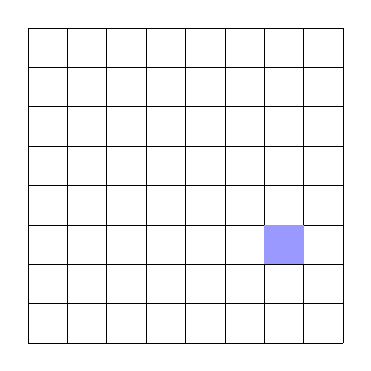
\begin{tikzpicture}
    \draw[step=0.5cm,black,very thin] (-2,-2) grid (2,2);
    \fill[blue!40!white] (1,-1) rectangle (1.5,-0.5);
  \end{tikzpicture}
\end{center}
Two people look at this board and decide to play a game. \\
One tells the other ``Let's take turns moving this knight towards the top left
of this board using only knight-like moves. If I am left with no
legal moves on my turn, I lose. If you can't make any move on your
turn, you lose'', and since she is bored, she readily agrees. \\
What can we say about this game? For clarity, the moves that the first
player can make are highlighted in red below. The the possible moves
for the rest of the game should be clear $\ldots$
\begin{center}
  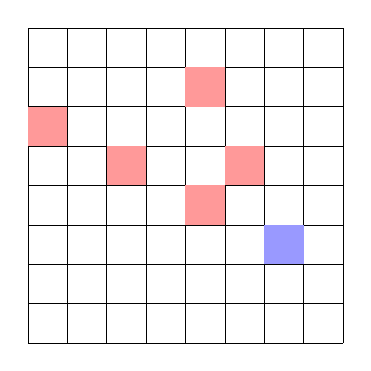
\begin{tikzpicture}
    \draw[step=0.5cm,black,very thin] (-2,-2) grid (2,2);
    \fill[blue!40!white] (1,-1) rectangle (1.5,-0.5);
    \fill[red!40!white] (0.5,0) rectangle (1,0.5);
    \fill[red!40!white] (0,1) rectangle (0.5,1.5);
    \fill[red!40!white] (0,-0.5) rectangle (0.5,0);
    \fill[red!40!white] (-1,0) rectangle (-0.5,0.5);
    \fill[red!40!white] (-2,0.5) rectangle (-1.5,1);
  \end{tikzpicture}
\end{center}
Observe that every square has a certain nimber, so \textit{ideally} we
should come up with a system to figure out the nimber given a
row, column pair. \\
For additional inspiration/motivation, a manually computed and 
color-coded diagram of the board is presented below:
\begin{center}
  \includegraphics[scale=0.2]{chessboardWithNimbers}
\end{center}
\paragraph{Claims to Prove}\mbox{}\\
Suppose we start numbering our rows and colums from $0$. Then, we can say:
\begin{enumerate}
  \item \textit{Claim:} The square at row $r$ and column $c$ has the same nimber
    as the square at row $c$ and column $r$.
  \item \textit{Claim:} Every square in row $r$, starting at column $2r$, 
    has nimber $r$.
  \item \textit{Claim:} Every square at row $o$, column $o$, where $o$ is any
    odd number, has nimber $0$.
  \item \textit{Claim:} Every square at row $e$, column $e$, where $e$ is any
    even number $\neq 4$, has nimber $1$. \\
    The square at row $4$, column $4$ has nimber $2$.
  \item \textit{Claim:} At row $r$, the squares at columns $(2r - 1)$ and
    $(2r - 2)$ both have nimber $(r - 1)$.
  \item \textit{Claim:} At row $r$, the square at column $(2r - 3)$
    has nimber $(r - 3)$ when $r$ is odd and $(r - 1)$ when $r$ is even.
  \item \textit{Claim:} At row $r$, the square at column $(2r - 4)$
    has nimber $(r - 2)$.
  \item \textit{Claim:} At row $r$, the square at column $(2r - 4)$
    has nimber $(r - 2)$.
\end{enumerate}
\paragraph{Proving Periodic Differences}\mbox{}\\
Suppose we have a zero-indexed game board where the top row and
leftmost columns both have index 0. \\
Let the function $N : \N^2 \rightarrow \N$ be the function that maps the
square $(r,c)$ to its nimber. \\
The hypothesis is that, for $i \geq 0$,
\begin{align*}
  N(6 + (i + 1), 6 + 2(i + 1)) - N(6 + i, 6 + 2i) =
  \begin{cases}
    3, & \text{if} \: i \equiv 0 \pmod{4} \\
    2, & \text{if} \: i \equiv 1 \pmod{4} \\
    1, & \text{if} \: i \equiv 2 \pmod{4} \\
    -2, & \text{if} \: i \equiv 3 \pmod{4}
  \end{cases} \\
  \R N(7 + i, 8 + 2i) - N(6 + i, 6 + 2i) =
  \begin{cases}
    3, & \text{if} \: i \equiv 0 \pmod{4} \\
    2, & \text{if} \: i \equiv 1 \pmod{4} \\
    1, & \text{if} \: i \equiv 2 \pmod{4} \\
    -2, & \text{if} \: i \equiv 3 \pmod{4}
  \end{cases}
\end{align*}
We can perform a quick sanity check using the code or the data in the
\verb|nimbers.numbers| file, to assert that we have framed the hypothesis
correctly:
\begin{align*}
  i = 0: &\: N( 7, 8) - N( 6, 6) = 3  = 4 - 1 \\
  i = 1: &\: N( 8,10) - N( 7, 8) = 2  = 6 - 4 \\
  i = 2: &\: N( 9,12) - N( 8,10) = 1  = 7 - 6 \\
  i = 3: &\: N(10,14) - N( 9,12) = -2 = 5 - 7 \\
  i = 4: &\: N(11,16) - N(10,14) = 3  = 8 - 5 \\
  i = 5: &\: N(12,18) - N(11,16) = 2  = 10 - 8 \\
  i = 6: &\: N(13,20) - N(12,18) = 1  = 11 - 10 \\
  i = 7: &\: N(14,22) - N(13,20) = -2 = 9 - 11
\end{align*}
Suppose that we're at square $(6 + 4i, 6 + 8i)$, where $i = 1$. \\
We want to show that $N(7 + 4i, 8 + 8i) = N(6 + 4i, 6 + 8i) + 3$. \\
Now $N(6 + 4i, 6 + 8i) = 1 + 4i$, so we need to show that
$N(7 + 4i, 8 + 4i) = 4(i + 1)$.
\newpage
We can assume the hypothesis holds for all the squares before
$(7 + 4i, 8 + 8i)$, and so we see that the following squares have the
following nimbers:
\begin{align*}
N(6 + 4i, 6 + 8i) & = 4i + 1 \\   
N(6 + 4i - 1, 6 + 8i - 2) & = 4i + 3 \\   
N(6 + 4i - 2, 6 + 8i - 4) & = 4i + 2 \\   
N(6 + 4i - 3, 6 + 8i - 6) & = 4i \\
N(6 + 4i - 4, 6 + 8i - 8) & = 4(i - 1) + 1 \\
N(6 + 4i - 5, 6 + 8i - 10) & = 4(i - 1) + 3 \\
N(6 + 4i - 6, 6 + 8i - 12) & = 4(i - 1) + 2 \\
N(6 + 4i - 7, 6 + 8i - 14) & = 4(i - 1) \\
\cdots \\
N(6 + 4i - 4i, 6 + 8i - 8i) & = 4(i - i) + 1 \\
N(5, 4) & = 3 \\
N(4, 2) & = 2 \\
N(3, 0) & = 0
\end{align*}
Since we can reach any one of these squares from square $(7 + 4i, 8 + 8i)$
in one single-up double-left move, $N(7 + 4i, 8 + 8i) > 4i + 3$. \\
Now the question is --- can we reach a square with nimber $4i + 3$ in
one double-up single-left move?
\begin{align*}
  N(5 + 4i, 7 + 8i) = 4i + 2 \\
  N(3 + 4i, 6 + 8i) = N(3 + 4i, 2 * (3 + 4i)) = 4i + 3 \\
\end{align*}
Since $(3 + 4i, 6 + 8i)$ is the very first square in the grid to have
the nimber $(3 + 4i)$, so all squares to its top-left will have a lesser
nimber. \\
This is a ``loose'' proof that $N(7 + 4i, 8 + 8i) = 4(i + 1)$.
\newpage
\paragraph{Proving Periodic Differences Better}\mbox{}\\
Suppose we have a zero-indexed game board where the top row and
leftmost columns both have index 0. \\
Let the function $N : \N^2 \rightarrow \N$ be the function that maps the
square $(r,c)$ to its nimber. \\
The hypothesis is that, for $i \geq 0$,
\begin{align*}
  N(4 + i, 2(i + 1)) - N(3 + i, 2i) =
  \begin{cases}
    2, & \text{if} \: i \equiv 0 \pmod{4} \\
    1, & \text{if} \: i \equiv 1 \pmod{4} \\
    -2, & \text{if} \: i \equiv 2 \pmod{4} \\
    3, & \text{if} \: i \equiv 3 \pmod{4}
  \end{cases}
\end{align*}
We can perform a quick sanity check using the code or the data in the
\verb|nimbers.numbers| file, to assert that we have framed the hypothesis
correctly:
\begin{align*}
  i = 0: &\: N(4,2) - N(3,0) = 2 \\
  i = 1: &\: N(5,4) - N(4,2) = 1 \\
  i = 2: &\: N(6,6) - N(5,4) = -2 \\
  i = 3: &\: N(7,8) - N(6,6) = 3 \\
  i = 4: &\: N(8,10) - N(7,8) = 2 \\
  i = 5: &\: N(9,12) - N(8,10) = 1 \\
  i = 6: &\: N(10,14) - N(9,12) = -2 \\
  i = 7: &\: N(11,16) - N(10,14) = 3
\end{align*}
Suppose we want to prove: \\
Note that
\begin{align*}
  &\: N(3+(4k),2\cdot(4k))-N(3+(4(k-1)),2\cdot(4(k-1))) \\
  = &\: \big(N(3+(4k),2\cdot(4k))-N(3+(4(k-1)+3),2\cdot(4(k-1)+3))\big) + \\
  &\: \big(N(3+(4(k-1)+3),2\cdot(4(k-1)+3))-N(3+(4(k-1)+2),2\cdot(4(k-1)+2))\big) + \\
  &\: \big(N(3+(4(k-1)+2),2\cdot(4(k-1)+2))-N(3+(4(k-1)+1),2\cdot(4(k-1)+1))\big) + \\
  &\: \big(N(3+(4(k-1)+1),2\cdot(4(k-1)+1))-N(3+(4(k-1)),2\cdot(4(k-1)))\big) \\
  = &\: 3 - 2 + 1 + 2 \\
  = &\: 4
\end{align*}
This tells us:
\begin{align*}
  N(3+(4k),2\cdot(4k)) = 4k + N(3,0) = &\: 4k + 0 = 4k \\
  N(3+(4k+1),2\cdot(4k+1)) = &\: 4k + 2 \\
  N(3+(4k+2),2\cdot(4k+2)) = &\: 4k + 3 \\
  N(3+(4k+3),2\cdot(4k+3)) = &\: 4k + 1
\end{align*}
\newpage
\paragraph{Proving a Needed Result}\mbox{}\\
Consider the ``diagonal''
\begin{equation*}
  D = \{(2+i,1+i) : i \geq 0\}
\end{equation*}
We can conjecture that for $i\geq0$:
\begin{equation*}
N(2+(i+1),1+2(i+1))-N(2+i,1+2i) =
\begin{cases}
  -1 & \text{when}\  i \equiv 0 \pmod{2} \\
  3 & \text{when}\  i \equiv 1 \pmod{2}
\end{cases}
\end{equation*}
Performing a sanity check:
\begin{align*}
  i = 0: &\: N(3,3) - N(2,1) = 0 - 1 = -1 \\
  i = 1: &\: N(4,5) - N(3,3) = 3 - 0 = 3 \\
  i = 2: &\: N(5,7) - N(4,5) = 2 - 3 = -1 \\
  i = 3: &\: N(6,9) - N(5,7) = 5 - 2 = 3 \\
  i = 4: &\: N(7,11) - N(6,9) = 4 - 5 = -1 \\
  i = 5: &\: N(8,13) - N(7,11) = 7 - 4 = 3 \\
  i = 6: &\: N(9,15) - N(8,13) = 6 - 7 = -1 \\
  i = 7: &\: N(10,17) - N(9,15) = 9 - 6 = 3
\end{align*}
This seems to work. \\
Consider a square $(2+(2i-1),1+2(2i-1))$ where $i \geq 1$. 
\end{document}
